%!TEX root = ../main.tex
\section{Case Study: The Matrix Square Root on Heterogeneous Platforms}
The square root of a matrix $A$ is any matrix $X$ which satisfies the equation $A=X^2$. When it exists, it is not unique. When $A$ has no real negative eigenvalues, it has a unique square root whose eigenvalues all lie in the open right half-plane (i.e.\ have nonnegative real parts) \cite[20]{Higham:2008:FM}. This is the so-called principal square root $A^{1/2}$ and plays a major role in applications. Therefore, we will be interested in computing such square root whenever it exists.



However, the \textit{principal square root} $A^{1/2}$ of the matrix $A$ is the unique square root for which every eigenvalue lie in the open right half-plane (i.e.\ has a nonnegative real part). $A$ is assumed to be square.

The Schur method of Björck and Hammarling \cite{Bjorck:Hammarling:1983} computes the square root of the matrix by reducing $A$ to the upper triangular form $T$ and solving
\begin{IEEEeqnarray}{rCl}
U_{ii}^2 & = & T_{ii}\enspace\mathrm{,}\IEEElabel{eq:sqrtm:diag}\\
U_{ii}U_{ij} + U_{ij}U_{jj} & = & T_{ij} - \sum^{j-1}_{k = i + 1}{U_{ik}U_{kj}}\enspace\mathrm{,}\IEEElabel{eq:sqrtm:ndiag}
\end{IEEEeqnarray}
where $U^2=T$, being $U$ also upper triangular. This is the most numerically stable method and it is implemented in MATLAB as the \texttt{sqrtm} and \texttt{sqrtm\_real} functions \cite{Higham:MFT}.

\Cref{eq:sqrtm:diag,eq:sqrtm:ndiag} describe an algorithm which can be computed a column, row or superdiagonal at a time.
While a column or row at a time is preferred for any serial implementation due to a more efficient use of cache memory, it prevents parallelism: each element depends on the ones on the left and below, as shown in \cref{fig:sqrtm:dependencies}.
On the other hand, all the elements in a superdiagonal depend only on those in the superdiagonals below, which allows to compute all elements in parallel.

\begin{figure}[!htp]
	\begin{center}
		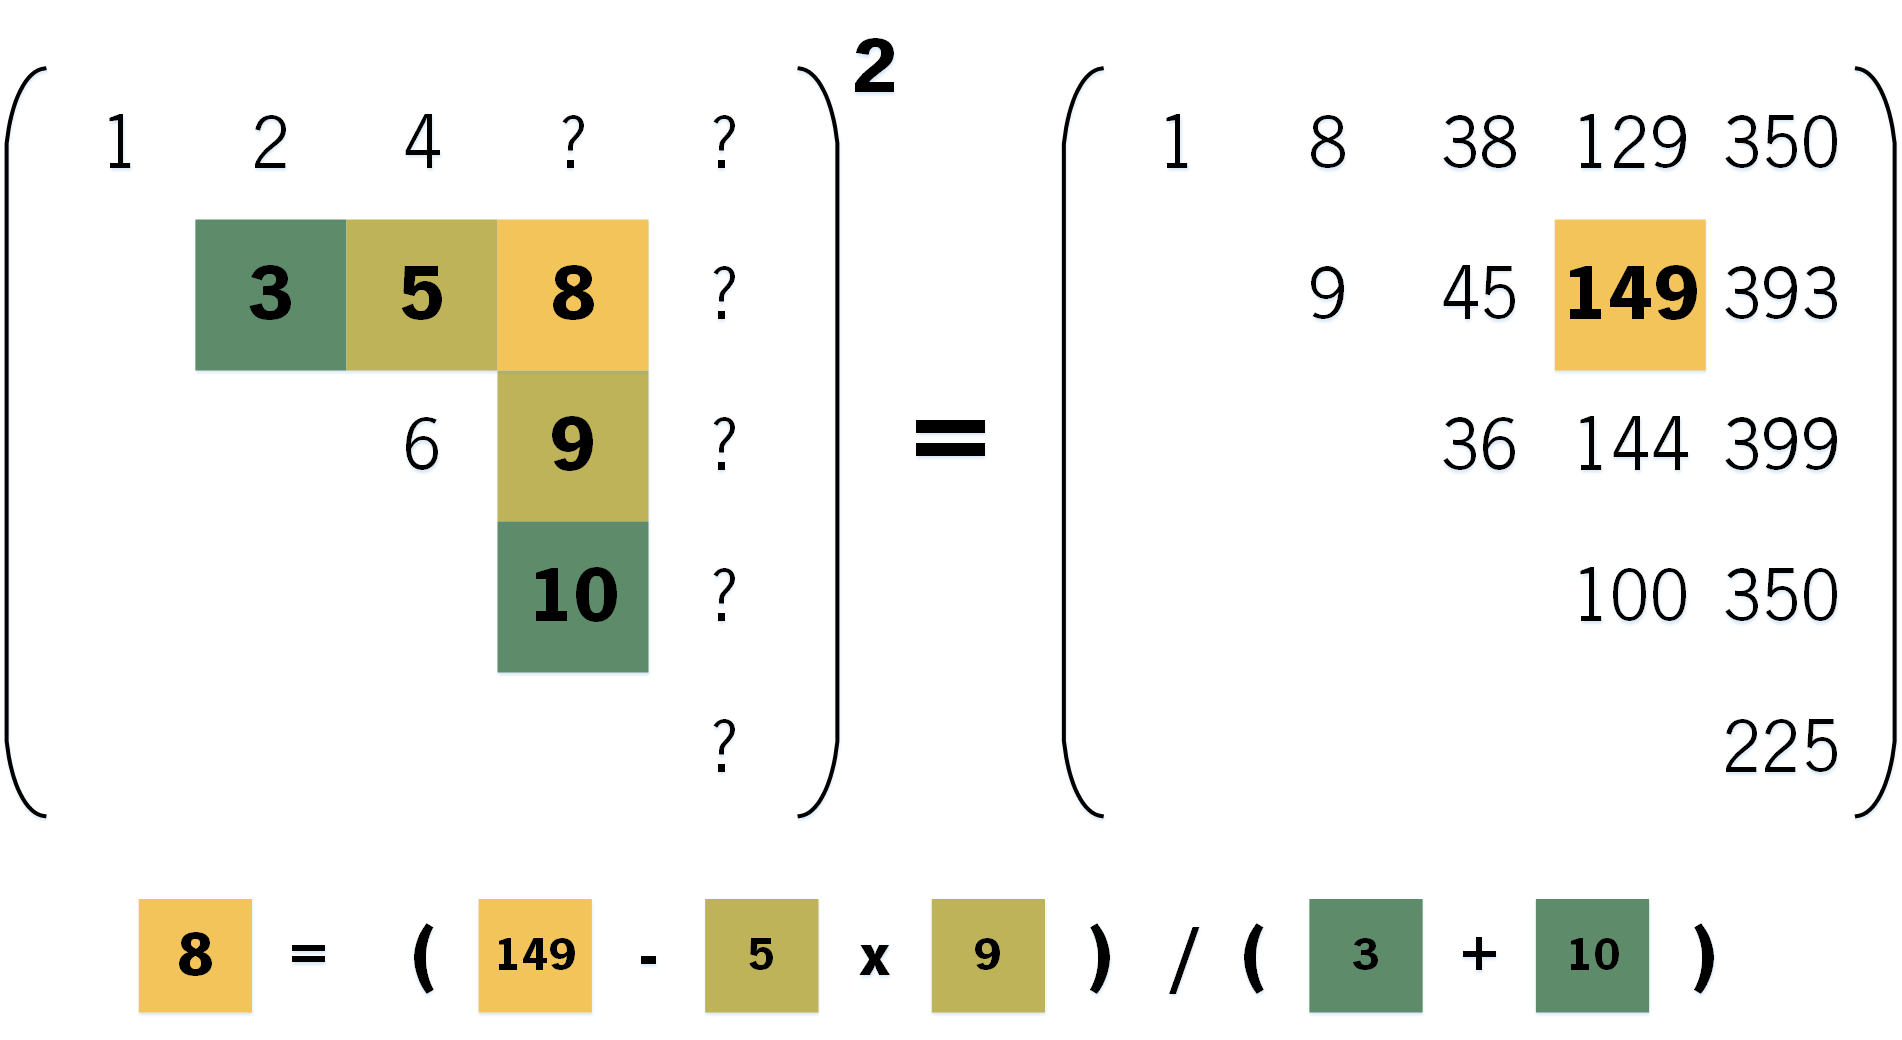
\includegraphics[width=.3\textwidth]{dependencies.png}
	\end{center}
	\caption[Algorithm dependencies]{The required elements to compute $U_{ij}$ in the Schur method of Björck and Hammarling.}
	\label{fig:sqrtm:dependencies}
\end{figure}
